\documentclass{report}
\usepackage{graphicx}
\usepackage{color}
\usepackage{array}
\definecolor{Green}{RGB}{100, 200, 45}
\definecolor{Blue}{RGB}{60, 0, 255}
\definecolor{Red}{RGB}{255, 0, 0}
\definecolor{Purple}{RGB}{60, 26, 78}
\definecolor{White}{RGB}{255, 255, 255}
\renewcommand{\chaptername}{Capitolo}
\renewcommand{\contentsname}{Indice}
\renewcommand{\figurename}{Immagine}
\graphicspath{ {/home/riky/Documents/Git/Clown-Fiesta-ICT/Reports/Relazione_Lavoro_Di_Gruppo/Immagini_Relazione/} }

\author{Catone Mario,\\
	Oglietti Riccardo,\\
	Serena Thomas,\\
Volgarino Livio}
\title{Relazione Lavoro Di Gruppo\\
\large Gruppo 2, Clown-Fiesta-ICT}
\date{\today}

\makeindex

\begin{document}
	\maketitle
	\tableofcontents
	\chapter{Introduzione}
	\author{Oglietti Riccardo}
		\section{La Sfida}
			Il progetto che mi accingo a descrivere e' nato come figlio del corso \emph{Learning By Project} a opera dei docenti 
			Bardi Laura Silvia e Blachietti Andrea. In esso ci e' stato richiesto di progettare una nuova infrastruttura di 
			rete atta a rimpiazzare l'intera infrastruttura di una scuola superiore Piemontese. La scuola e' divisa in due 
			gruppi di edifici, i quali contengono le sedi di tre differenti indirizzi: \textbf{Liceo Scientifico delle Scienze 
			Applicate a Indirizzo Informatico}, \textbf{Istituto Tecnico Economico} e infine \textbf{Liceo Linguistico}.

			Entrambi i gruppi di edifici sono composti da tre piani, il primo gruppo e' formato da tre edifici, in due 
			dei quali sono concentrate aule, laboratori e locali amministrativi. Nella terza e' poi disposta la palestra
			e relativi locali.

			Il seconodo gruppo, non contiguo al primo, e' invece formato da due edifici, nel quale sono dislocate le aule e 
			i laboratori dell'Istituto Tecnico Economico, mentre nel seconodo e' presente la palestra e alcuni edifici
			amministrativi.

			La progettazione e' stata portata avanti tenendo conto di alcuni punti fondamentali, quali la necessita' di 
			fornire scalabilita' e facilita' di manutenzione da parte dei tecnici presenti all'interno dell'infrastruttura 
			scolastica, e la necessita' di un controllo capillare della sicurezza tramite l'utlizzo di alcuni strumenti 
			fondamentali quali l'infrastruttura MS Active Directory e l'utilizzo di firewall integrati con essa. 

			Un'altra sezione sicuramente fondamentale del progetto e' sicuramente quella legata all'organizzazione di un 
			gruppo di lavoro il piu' efficiente e produttivo possibile, atto a risolvere un problema complesso nella sua 
			struttura. Cio' ci ha permesso di venire in contatto con alcune delle piu' comuni difficolta' del lavoro di
			gruppo
			e di imparare molto su come gestirle, inoltre, trattandosi del primo vero progetto di gruppo per molti di noi 
			l'entusiasmo si e' dimostrato molto fin dalla prima lezione.

		\section{Il Team}
			Il gruppo classe e' stata suddivisa in sette differenti gruppi, il nostro gruppo, il numero due, e' formato dai 
			seguenti studenti:
			\begin{itemize}
				\item \textbf{Catone Mario}
				\item \textbf{Oglietti Riccardo}
				\item \textbf{Serena Thomas}
				\item \textbf{Volgarino Livio}
			\end{itemize}
			Durante l'organizzazione del progetto abbiamo optato per suddividere le mansioni principalmente in base agli
			interessi e alle passioni dei singoli componenti, in maniera da rendere lo sforzo collettivo quanto piu'
			produttivo possibile. 

			In merito all'organizzazione interna non possiamo dire di aver definito una gerarchia o un vero e proprio 
			"Team Leader", bensi' di esserci organizzati come pari, affidando un carico il piu' possibile uniforme in 
			termini di iportanza e impegno richiesto.

	\chapter{Organizzazione E Strumenti}        
		\section{Comunicazione}
			Come primo passo, durante il primo incontro abbiamo cercato di definire una selezione di strumenti atti a 
			gestire una serie di apetti fondamentali delle dinamiche insite nel teamwork, in primis la Comunicazione
			tra collghi.
			La nostra scelta si e' orientata verso alcuni strumenti chiave: innanzitutto abbiamo optato per la scelta
			della piattaforma \emph{Telegram} per la messaggistica istantanea e le comunicazioni piu' rilevanti grazie
			alle ampie possibilita' di gestione del gruppo, quale la possibilita' di rendere un messaggio prioritario o
			evidenziato. Abbiamo poi deciso di usare lo strumento \emph{GIT} per coordinare la gestione dei documenti
			prodotti da ogni membro del gruppo. Infine, abbiamo optato per lo strumento di conferenza \emph{Discord} per
			gestire gli incontri in remoto al di fuori dell'orario scolastico.
		\section{Strumenti Tecnici}
			La selezione degli stumenti tecnici si e' invece rivelata piu' ardua, l'ostacolo piu' grande e' stato coordinare
			le necessita' di ognuno all'interno di un set di strumenti congruo agli obbiettivi del progetto.
			Per quanto riguarda la stesura di relazioni e documenti, abbiamo optato per l'utilizzo del linguaggio \LaTeX:
			esso permette di strutturare documenti estremamente complessi mantenendo una relativa semplicita' di utilizzo.
			Inoltre l'integrazione con lo strumento di sviluppo collaborativo \emph{git} e' ottima, e ha permesso di
			ottimizzare lo sforzo comune. Da notare poi la possibilita' di gestire i documenti tramite il comodo sistema
			basato su commit sul quale si basa \emph{git}, e' stato largamente piu' semplice gestire le revisioni
			collaborative per qualsivoglia documento, e la scrittura collaborativa, indispensabile per la redazione delle
			relazioni.
			Per cio' che concerne invece la creazione di diagrammi di rete, e' stato scelto lo strumento gratuito
			\emph{Draw.io}: si tratta di una Webapp atta a creare rappresentazioni grafiche di qualsiasi genere.
			Il tool e' stato scelto per via della sua semplicita' d'uso e della possibilita' di esportare liberamente
			i documenti creati.
		\section{Definizione Dei Ruoli}
			Infine, abbiamo deciso di operare alcune scelte organizzative a nostro avviso opportune per poter gestire il
			progetto nella sua interezza. Abbiamo optato per un organizzazione basata su una suddivisione in ruoli, con
			mansioni specifiche e mediamente lunghe, per poi coordinare gli sforzi durante meeting con cadenza settimanale.
			Per facilitare la nostra organizzazione interna abbiamo da subito deciso di assegnare un colore a ogni membro,
			tramite questo espediente ci e' stato piu' facile organizzare il lavoro e i compiti di ognuno in maniera chiara
			e visuale. 
			La suddivisione e' quindi risultata come segue:
			\begin{center}
				\begin{tabular}{ |c|c| }
					\hline
					Nome Componente & Compito Assegnato \\
					\hline \hline
					\textcolor{Blue}{Catone Mario} & \textcolor{Blue}{Active Directory} \\
					\hline
					\textcolor{Purple}{Oglietti Riccardo} & \textcolor{Purple}{Reportistica e presentazione} \\
					\hline
					\textcolor{Red}{Serena Thomas} & \textcolor{Red}{Firewall e sicurezza} \\
					\hline
					\textcolor{Green}{Volgarino Livio} & \textcolor{Green}{Topoogia di rete e routing} \\
					\hline
				\end{tabular}
			\end{center}
			Questa particolare suddivisione dei ruoli e' nata dopo un confronto sulle nostre tematiche di interesse, e sui
			nostri punti di forza principali. Per citare un esempio, \textcolor{Blue}{Catone Mario} ha scelto la sua mansione
			dopo aver seguito con interesse il corso proposto per l'amministrazione di sistemi basati su \emph{Windows e MS
			Active Directory} di Cristante Fabrizio e aver riscontrato un grande interesse sulla te-\\matica. Invece,
			\textcolor{Red}{Serena Thomas}, rimasto molto colpito dalle implicazioni legate alla sicurezza studiate e
			sperimentate durante il corso di \emph{Firewall} a opera di Vedovato Alberto, ha deciso di intraprendere
			questa mansione.

	\chapter{Diagramma Di Rete e Topologia}
	\begin{sloppypar}
		\author{Volgarino Livio}
		\section{La Struttura In Generale}
			Come precedentemente specificato, la struttura di rete e' stata ideata principalmente da Volgarino Livio, ed e
			implementata dedicando particolare attenzione ad alcuni aspetti giudicati pilastri fondamentali del progetto:
			\begin{itemize}
				\item La separazione delle reti: e' stato scelto di progettare due reti separate e largamente indipendenti
					in modo da rendere piu' agevole l'installazione e il mantenimento, inoltre un eventuale fallimento
					dell'infrastruttura in uno dei due edifici non penalizzerebbe la didattica all'interno del secondo plesso.
				\item L'utilizzo di indirizzamento statico per i dispositivi fissi, propri dell'istituto (quali, per esempio,
					postazioni all'interno dei laboratori informatici in ambo i plessi), estremamente utile per mantenere un'
					estrema semplicita' di gestione e di troubleshooting.
				\item Filtraggio di tutto il traffico da parte di router/firewall che agiscono da endpoint per ognuno dei due
					plessi, cio' permette di innalzare lo standard di sicurezza, in quanto tutto il traffico nella sua interezza
					viene analizzato.
				\item Connessione dei due plessi tramite l'ausilio di una \emph{VPN} gestita da due \emph{New Generation
					Firewall}, che fungono anche da endpoint per entrambe le reti.
			\end{itemize}
			Andremo ora a spiegare nel dettaglio l'architettura, aiutati dal diagramma di rete redatto tramite il precedentemente
			citato strumento di creazione grafici e diagrammi \emph{Draw.io}.
		\section{Il Diagramma}
			La rete nel suo complesso puo' essere riassunta tramite l'ausilio del seguente diagramma:

			\begin{figure}[h]
				\centering
				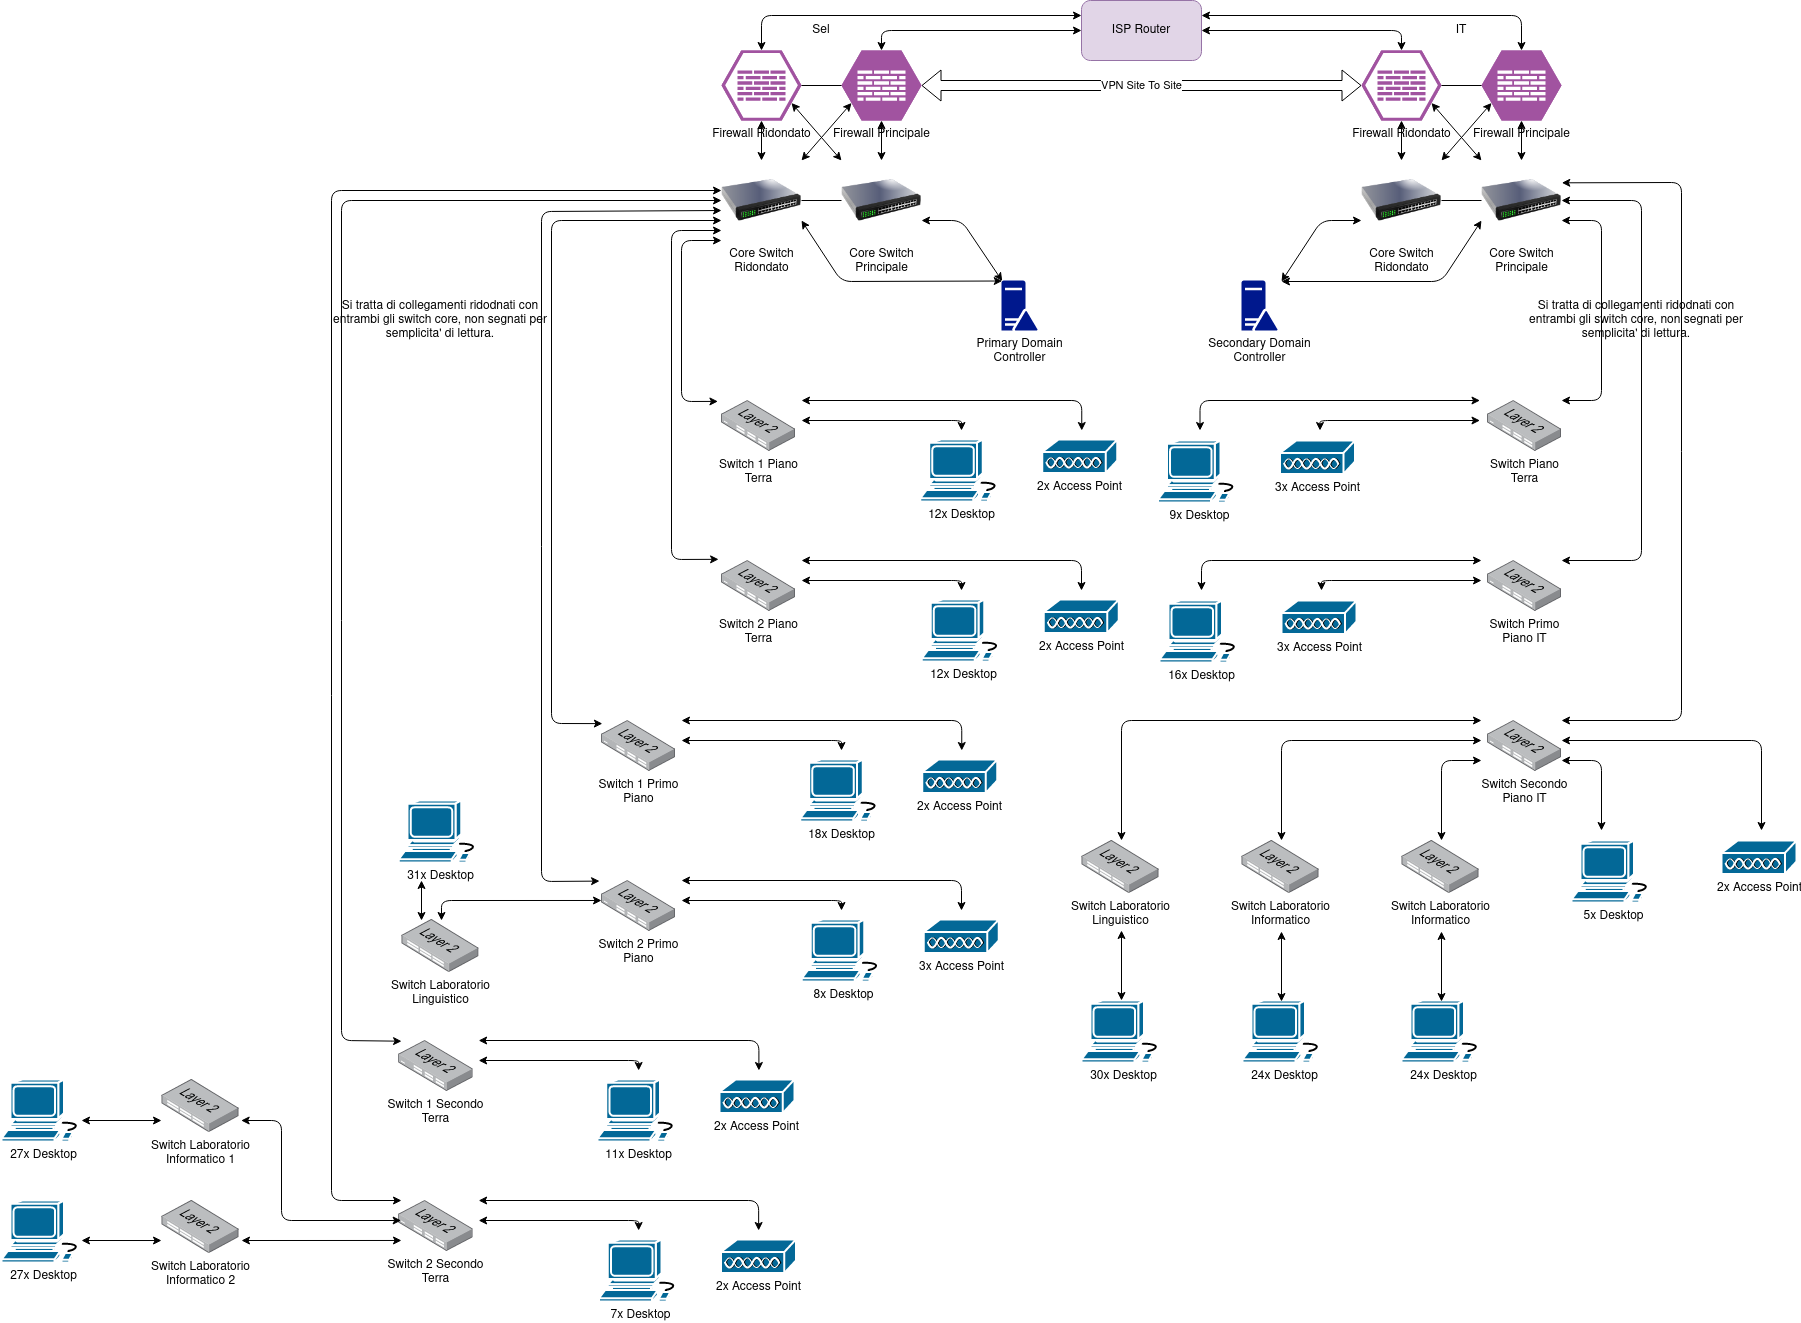
\includegraphics [width=\textwidth] {Schema_Di_Rete_Completo_1.png}
				\caption{Topologia di rete per ambo i plessi scolastici.}
				\label{fig:Diagramma Di Rete}
			\end{figure}
			Partendo dall'alto, possiamo subito notare la disposizione e la configurazione dei \emph{New Generation Firewall},
			data l'enorme importanza che ricoprono all'interno della nostra infrastruttura, abbiamo deciso di optare per la
			ridondanza dell'intera macchina fisica, cio' permette di mitigare qualsiasi problema di compromissione anche
			fisica dell'apparato. Data la complessita' del soggetto, abbiamo deciso di dedicare una sezione a parte
			all'argomento \textit{gestione \emph{New Generation Firewall e VPN} } durante un successivo capitolo.

			Un approccio simile e' stato adottato anche per quanto riguarda la gestione dei \emph{Core Switch}, essendo il
			cardine della rete per quanto riguarda l'instradamento dei pacchetti, e' stato scelto di ridondarli fiscamente
			permet-\\tendo quindi una piu' elevata tolleranza ad eventuali guasti.

			In generale, l'intera struttura di rete e' gerarchica, composta da un massimo di tre livelli. Il primo e'
			rappresentato dai due \emph{Core Switch} appena descritti, poi seguono un numero di apparati di \textit{"Secondo
			Livello"} pari a sei nel primo plesso e a tre nel seconodo. Per terminare con alcuni \emph{Switch} interni ai 
			vari laboratori, denominati come di \textit{"Terzo Livello"}. Per una questione di praticita' nell'illustrazione,
			abbiamo tracciato solamente i collegamenti tra ogni \emph{Switch} di \textit{"Secondo Livello"} e uno dei due 
			\emph{Core Switch}. Il grafico e' quindi da intendersi con un altro set di collegamenti tra ogni \emph{Switch}
			ed entrambi i \emph{Core Switch}, in maniera da poter rentere utile la ridondanza esplicata nel precedente
			paragrafo.

			Continuando verso il basso, possiamo notare il posizionamento dei due \emph{Domain Controller}, collegati
			direttamente con entrambi i \emph{Core Switch} in maniera da poter mantenere la continuita' del servizio a 
			prescindere dallo switch in uso in quel momento. Per via della necessita' di contenere i costi, abbiamo optato per
			non ridondare fisicamente tutte le macchine al di sotto del \textit{"Secondo Li-\\vello"}. Cio' ovviamente potrebbe
			compromettere l'accesso ad \emph{Active Direcory} a tutta l'area coperta da uno switch di \textit{"Secondo"} o
			\textit{"Terzo"} livello.

			Sullo schema di rete e' poi illustrato il numero di postazioni \emph{Desktop} collegati allo \emph{Switch}, 
			insieme al numero di \emph{Access Point} atti a creare un uniforme copertura wireless per l'interezza di
			entrambi i plessi.

			Per quanto riguarda la rete wireless in istituto, e' stato scelto di isolare tutti i device \textit{"Ospiti"}, ossia
			non connessi tramite rete cablata, su una \emph{Vlan} differente rispetto al resto dei dispositivi. Questa scelta 
			e' stata operata alla luce delle possibili falle di sicurezza che comporterebbe introdurre apparecchiature 
			esterne all'infrastruttura su una rete interna.
			E' infine necessario spendere qualche parola sulla disposizione fisica all'interno dei due plessi scolastici di
			tutti gli apparati. Abbiamo optato per il posizionamento di tutti gli \emph{Switch} si \textit{"Secondo Livello"}
			all'interno di appositi armati posizionati strategicamente all'interno dei corridoi dei piani assegnati. Cio'
			permette di mantenere uno standard di sicurezza elevato, in quanto sorvegliati da tutti gli insegnanti presenti 
			durante le pause nei corridoi. E' poi semplice cestire la cablatura degli edifici tramite la constrosoffittatura
			e l'aggiunta di canaline sospese dove necessario.
			Per quanto riguarda gli \emph{Access Point}, abbiamo deciso di posizionarli come in Figura
			\ref{fig:Diagramma Access Point IT} e in Figura \ref{fig:Diagramma Access Point SEL}:

			\begin{figure}[ht]
				\center
				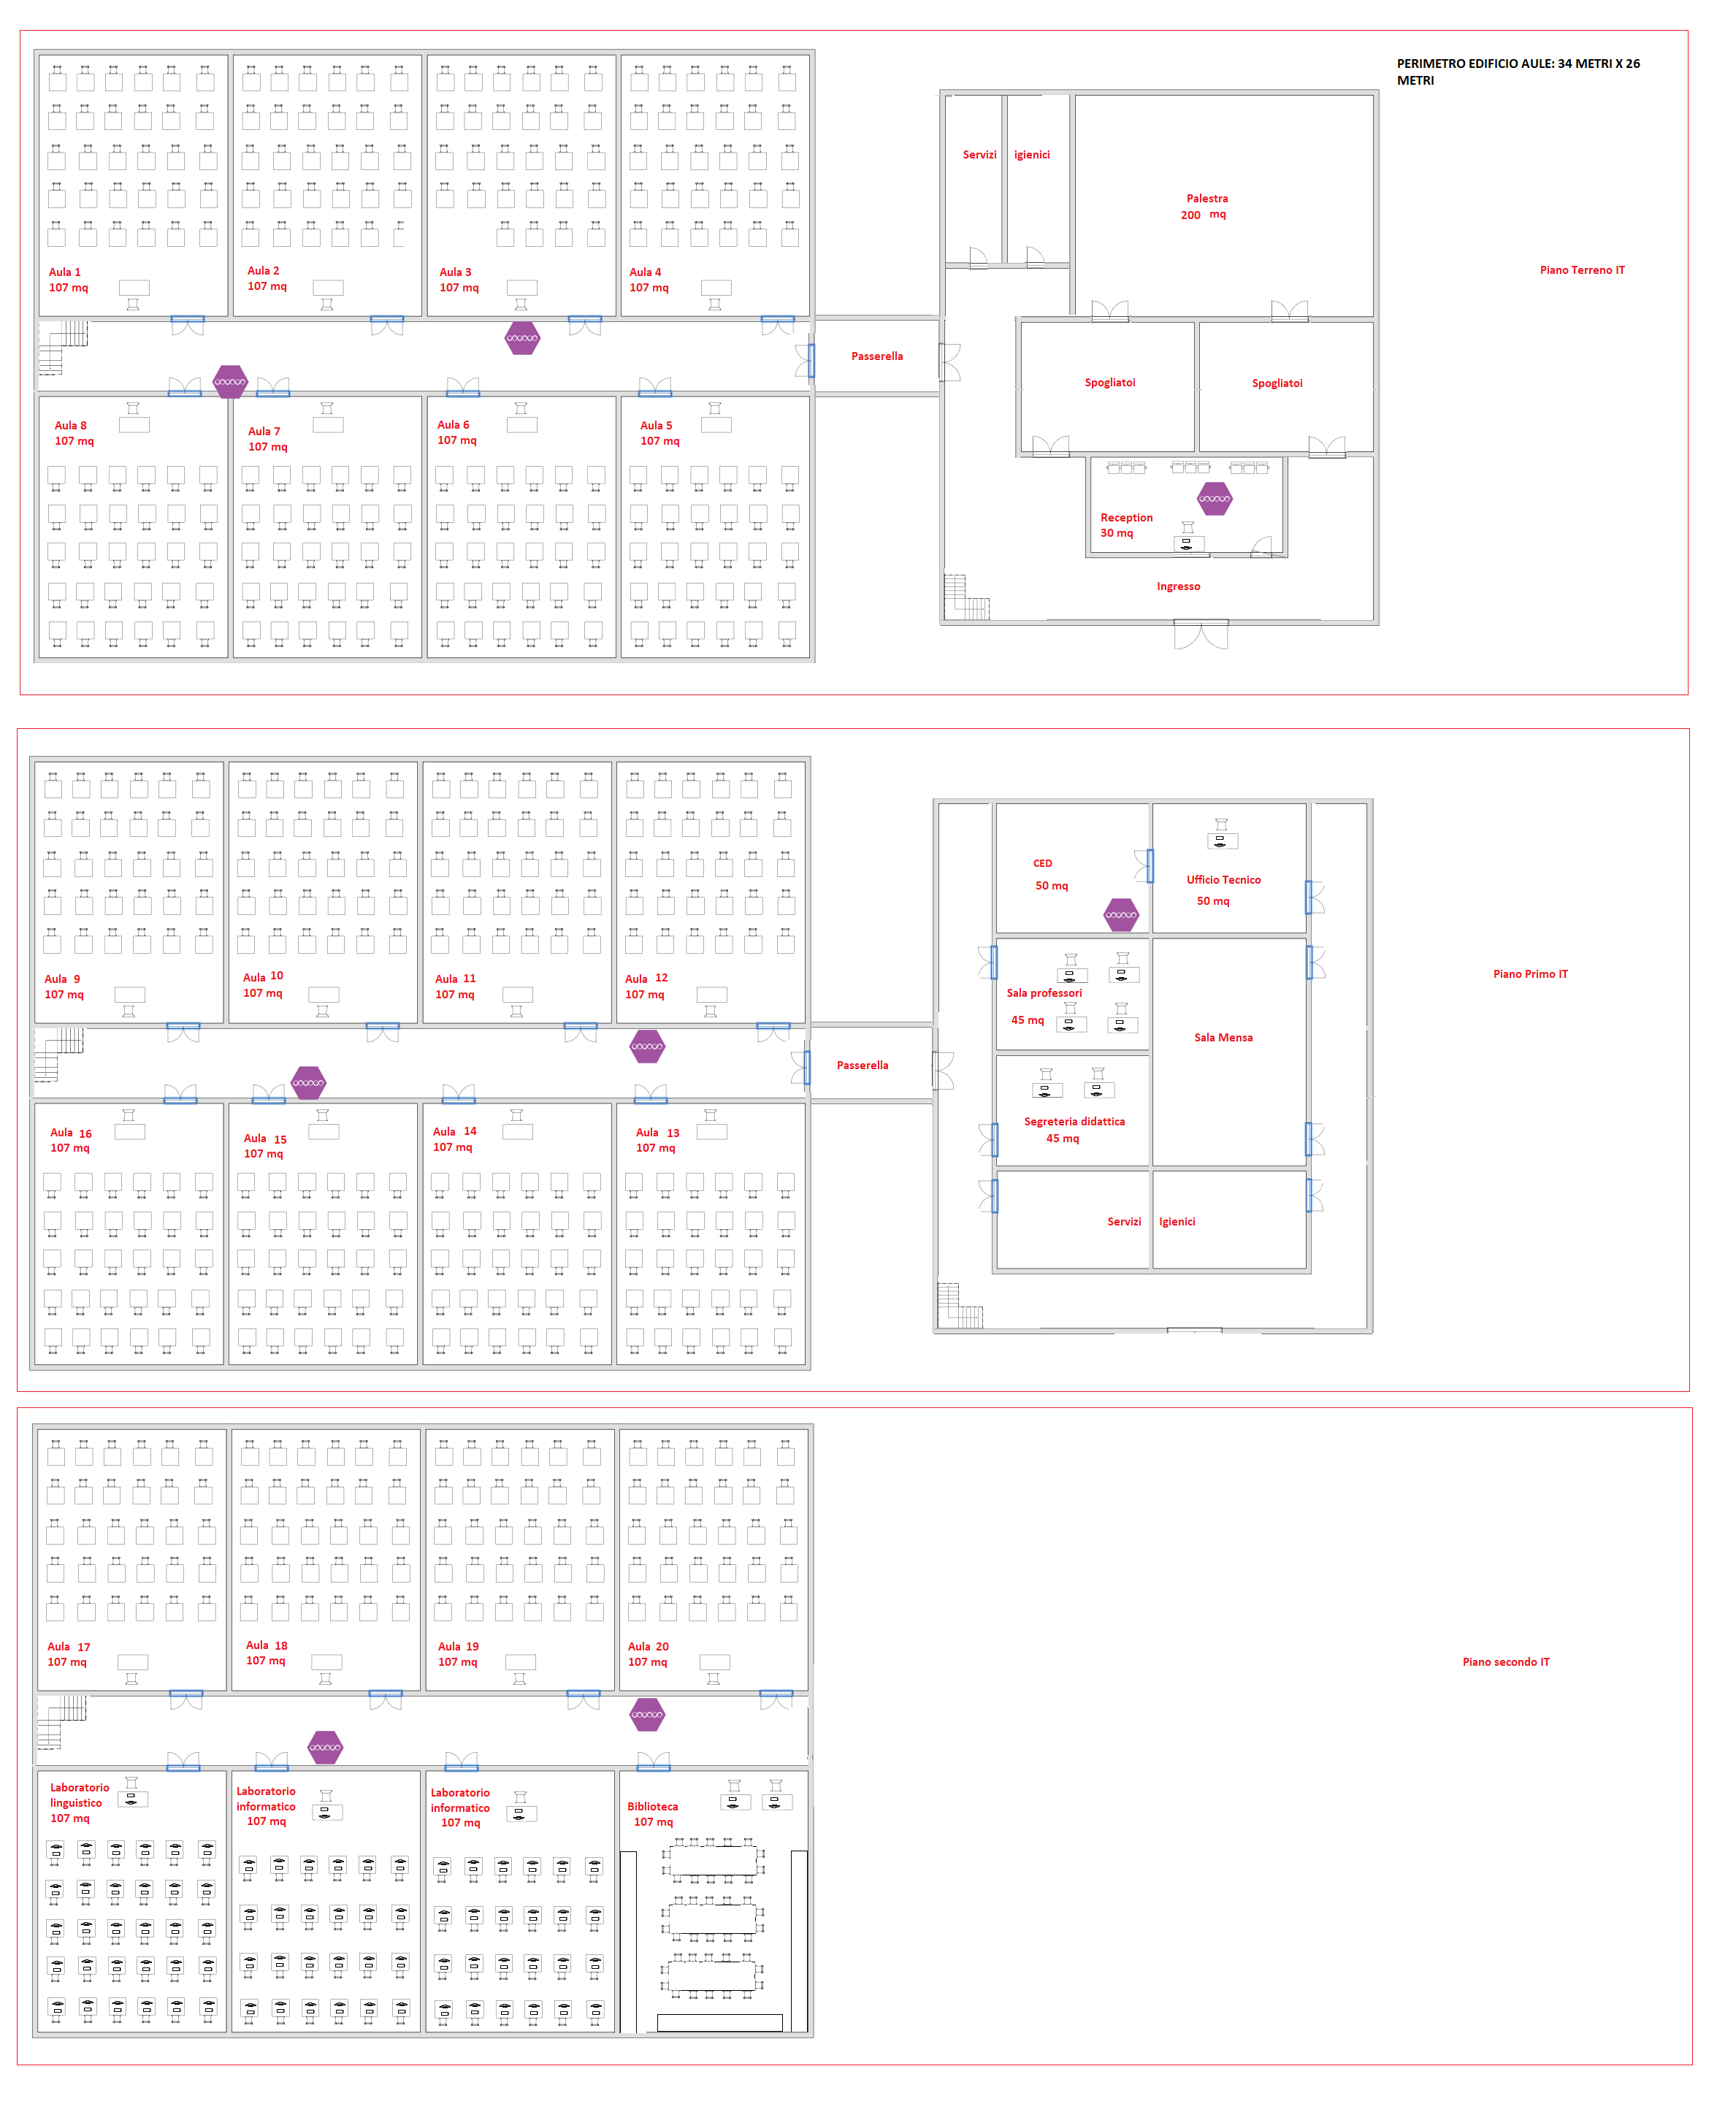
\includegraphics [scale=0.07, angle=90] {Posizione_AP_IT.png}
				\caption{Posizionamento Degli Access Point Plesso IT.}
				\label{fig:Diagramma Access Point IT}
			\end{figure}
			\begin{figure}[ht]
				\center
				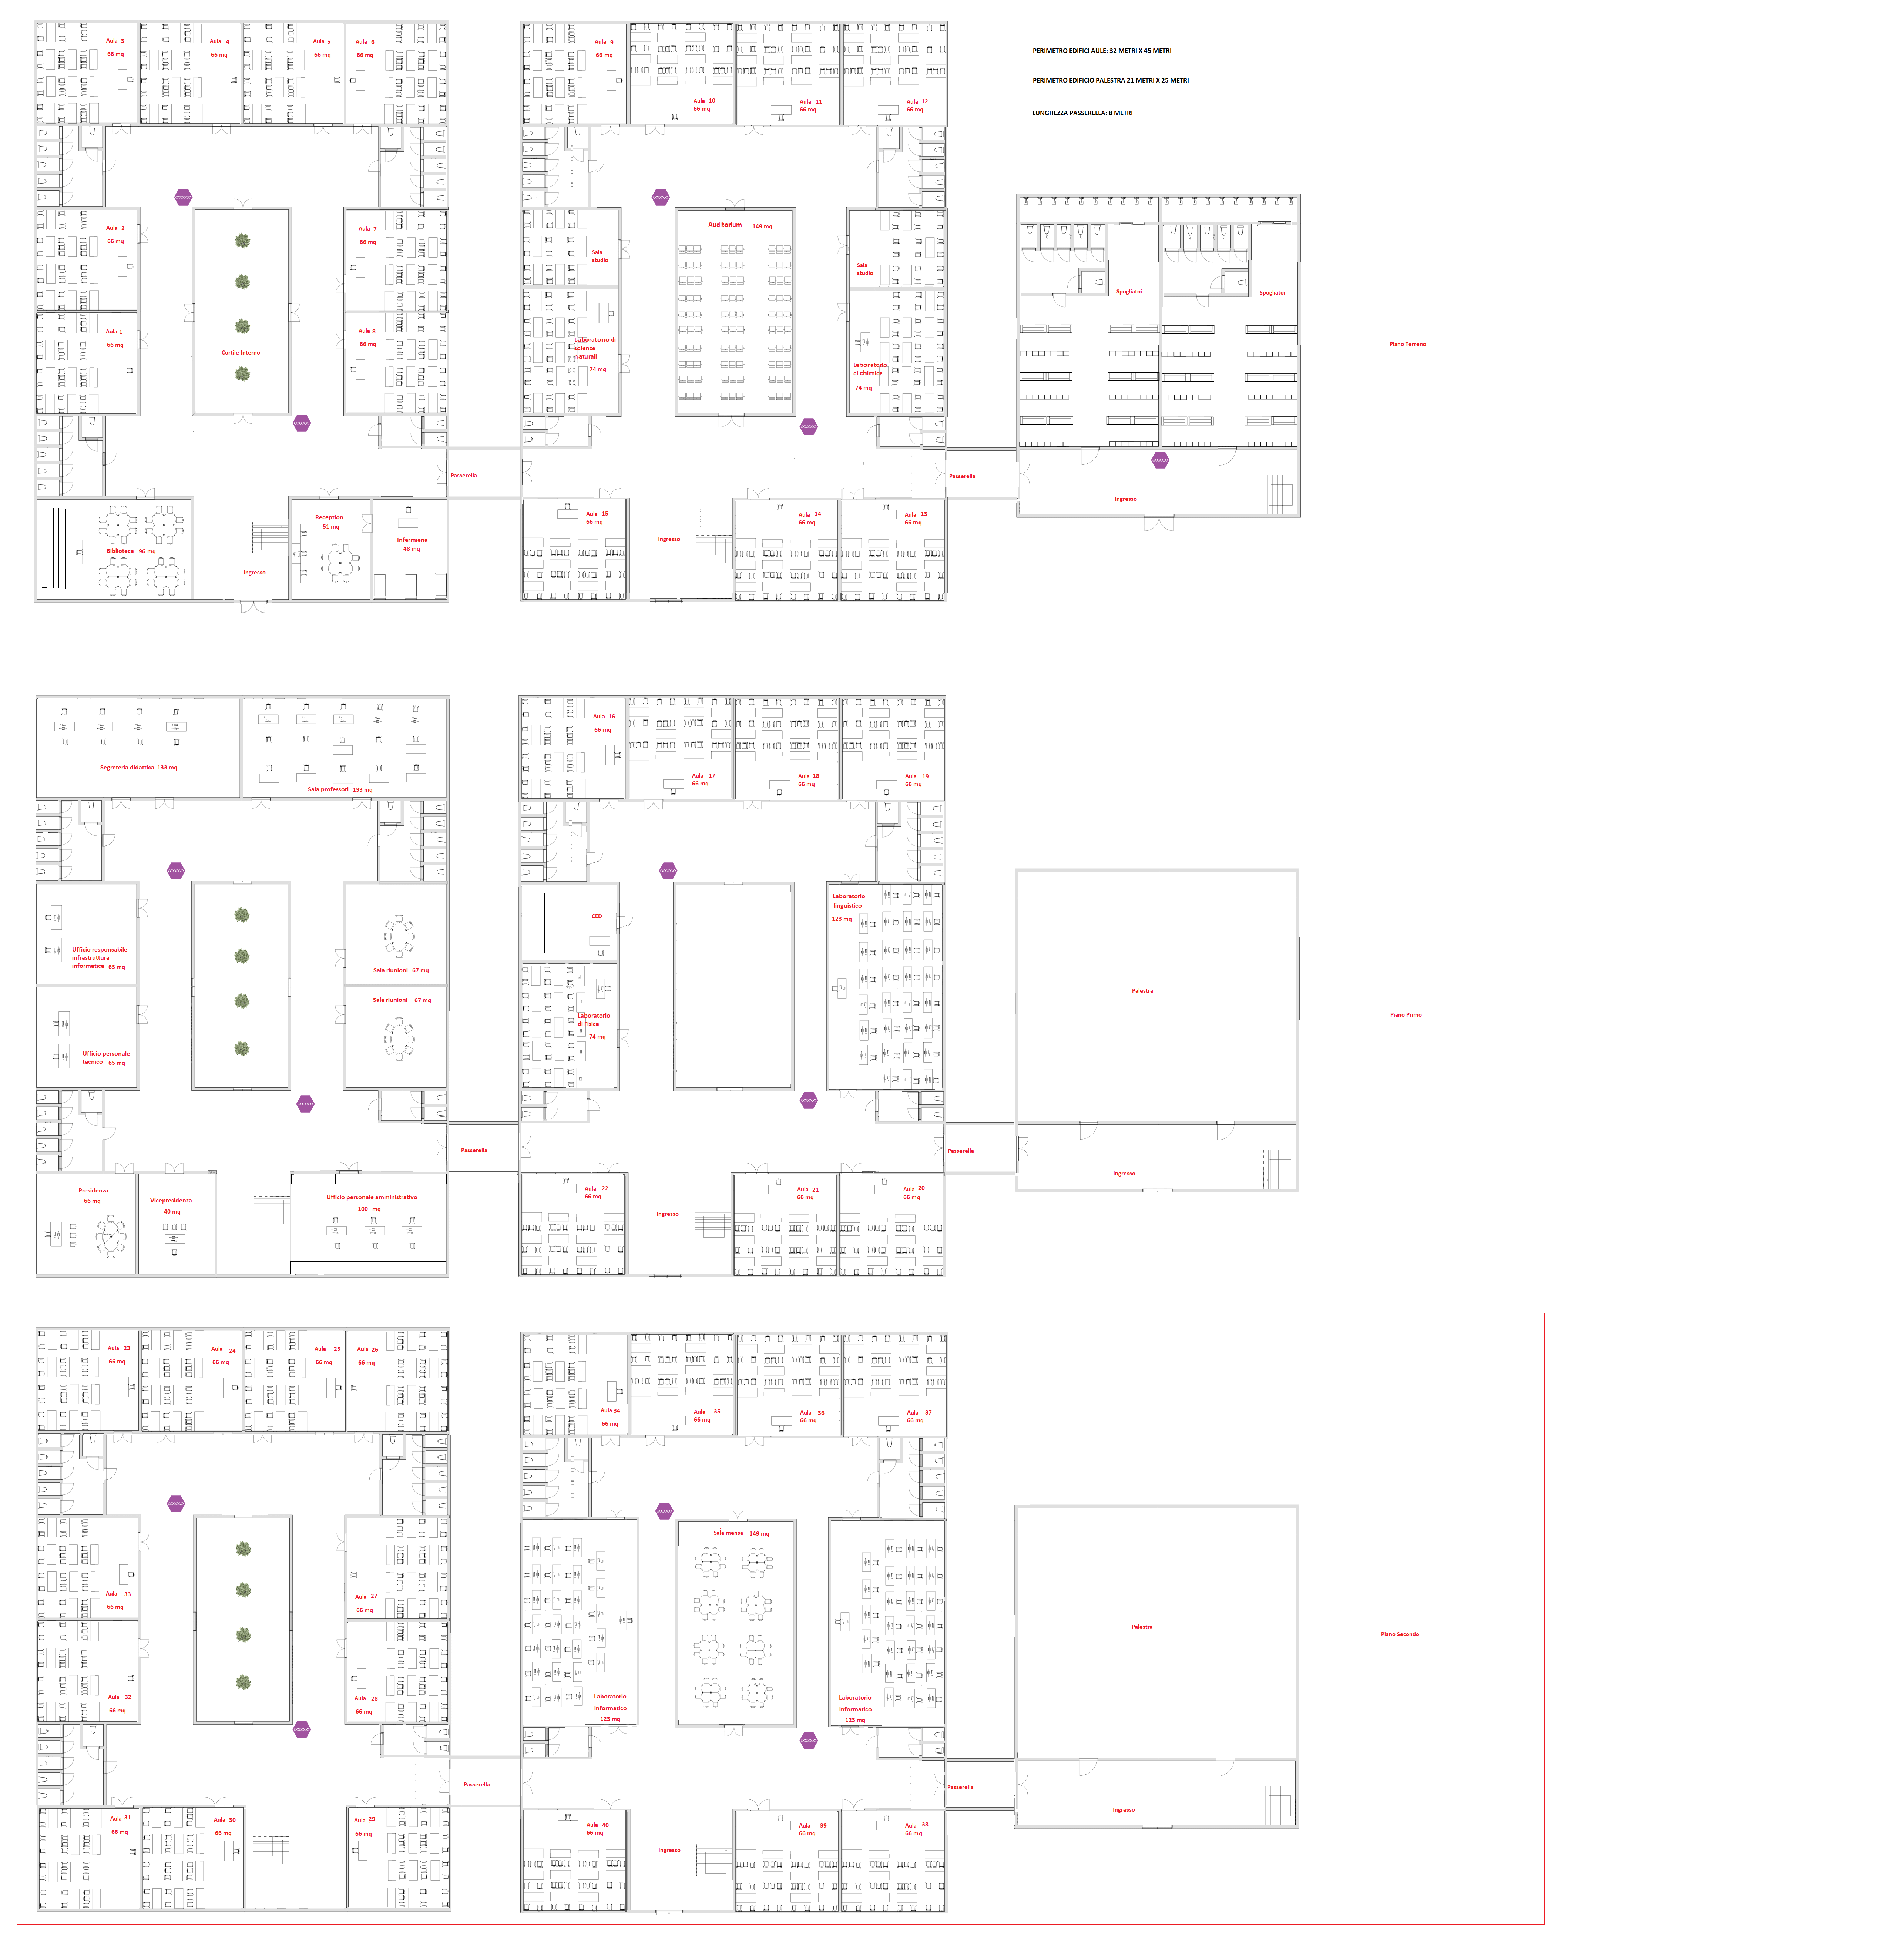
\includegraphics [scale=0.06, angle=90] {Posizione_AP_SEL}
				\caption{Posizionamento Degli Access Point Plesso SEL.}
				\label{fig:Diagramma Access Point SEL}
			\end{figure}
			\textcolor{White}{.}

			La disposizione e' stata ideata tentendo a mente la portata massima degli \emph{Access Point} da noi scelti
			(45 M), e la posizione di eventuali barriere architettoniche come muri in cemento o colonne portanti, che
			influenzerebbero negativamente la portata del segnale.
	\end{sloppypar}
	\chapter{Sicurezza E Firewall}
	\author{Serena Thomas}
		\section{Introduzione All'Infrastruttura}
			Come precedentemente specificato, per la gestione \emph{Firewall} abbiamo optato per il depoloy di un totale di
			quattro macchine fisiche, ridondate due a due. Essendo esse gli endpoint di entrambe le reti semi-indipendenti 
			presenti nei due plessi scolastici, assicurarne il corretto funzionamento e' essenziale per poter mantenere
			il servizio.
			I firewall sono direttamente connessi con il provider tramite connessione a 1GBPS, essi svolgono sia la funzione 
			di \emph{Router} che di \emph{Firewall}, esploreremo piu' avanti questo argomento con esaustivita'.

			Le mansioni principali che il \emph{Firewall} si trovera' a svolgere sono le seguenti:
			\begin{enumerate}
				\item Instradamento Pacchetti.
				\item Policy Per La Navigazione.
				\item Fornitura Indirizzi IP.
				\item Tunnel VPN.
			\end{enumerate}
		\section{Aspetti Principali}
			\subsection{Instradamento Pacchetti}
				Come annunciato in precedenza, i due \emph{Firewall} si andranno a posizionare a sostituzione degli apparati
				che normalmente assolverebbero alla funzione di \emph{Router} in modo da avere un solo dispositivo che svolga
				più mansioni: in questo modo, verra' sia ridotta la latenza introdotta da un analisi del traffico posteriore,
				sia l'ingombro fisico degli apparati, semplficando dunque la manutenzione e l'organizzazione.

				Per svolgere questo compito verranno introdotte delle \emph{Tabelle di Routing} nella configurazione delle due
				macchine in modo che queste sappiano dove inoltrare ogni singolo pacchetto con un determinato indirizzo IP.
			\subsection{Policy Di Navigazione e Autenticazione}
				Un altro aspetto della configurazione dei due \emph{Firewall} riguarda le \emph{Policy} di navigazione: il
				principio e' quello di creare \emph{Policy} differenziate a seconda del gruppo al quale afferisce ciascun utente 
				che sta navigando attraverso la rete scolastica. Verranno quindi create \emph{Policy} specifiche per studenti,
				docenti, personale (amministrativo e ATA) ed ospiti con differenti limitazioni in base a determinate categorie
				di siti web. Saranno per tutti bloccate alcune categorie di contenuti non ritenute consone ad un ambiente
				scolastico, (ad esempio alcool, droghe e pornografia) inoltre alcune non ritenute utili o potenzialmente
				dannose ai fini dell'apprendimento o della sicurezza, ad esempio (Intrattenimento e hacking).
				Alcuni siti e piattaforme come i vari social network, Netflix, Twitch e assimilabili saranno bloccati
				indipendentemente dall'utenza (in modo da evitare che vengano consultati tramite la rete scolastica in orario
				non consono) ma, nel caso nel quale ci siano richieste particolari, potra' essere concessa maggiore liberta' di
				navigazione ad alcune categorie di utenti, cio' allo scopo di permettere al corpo docente di poter trasmettere
				contenuti educativi agli studenti.

				La gestione dell’autenticazione e della conseguente applicazione della \emph{Policy} corretta al soggetto
				autenticato verra' gestita attraverso i server \emph{Active Directory}: nel momento in cui un utente tentera'
				di effettuare del traffico internet, apparira' un pop-up che richiederà l’inserimento delle proprie
				credenziali di dominio (o le credenziali da ospite fornite presso la reception) e i \emph{Firewall}
				si occuperanno di interrogare i server di autenticazione per sapere se quell’utenza e' legittimata
				ad effettuare traffico all’interno della rete scolastica e, nel caso in cui lo sia, quali tipi di
				piattaforme potra' visitare basandosi sulla \emph{Policy} collegata al suo gruppo di
				appartenenza.
			\subsection{Fornitura Indirizzi IP}
				Una delle principali mansioni dei \emph{Firewall} e' la fornitura di \emph{Indirizzi IP} ai dispositivi che ne
				fanno richiesta attraverso la configurazione del servizio \emph{DHCP}. Si e' scelto di avere un piano di
				indirizzamento fisso per quanto riguarda i dispositivi interni alle sedi connessi via cavo, mentre di
				fornire indirizzi variabili ai dispositivi ospiti: in questo modo i \emph{Firewall} dovranno gestire le
				richieste \emph{DHCP} di un numero limitato di dispositivi collegati alla rete e, in caso di bug o
				problemi di sorta, il troubleshooting sara' notevolmente piu' agile, in quanto l'identificazione
				del dispositivo sara' univoca rispetto al dipositivo.
			\subsection{Tunnel VPN}
				Infine, per mettere in comunicazione le due sedi e' stato pensato di intrudurre un \emph{Tunnel VPN}
				tra le interfacce esterne dei \emph{Firewall}: in questo modo il traffico che e' diretto da una sede
				all’altra sara' instradato all’interno di questo tunnel virtuale e viaggera' attraverso internet in
				totale sicurezza da un edificio all’altro. La necessita' di questo collegamento si puo' ricercare nella
				necessita' di mettere in collegamento i due \emph{Domain Controller}, in questo modo essi possono mantenere
				sincronizzazione tra loro, e in caso di failure tecnico di una delle due macchine, garantire almeno parte 
				del servizio ad entrambi i gruppi di edifici.
				La tabella riportata di seguito mostra i parametri utilizzati per la configurazione del \emph{Tunnel VPN} tra le
				due sedi.
				\begin{center}
					\begin{tabular}{ |c||c||c| }
						\hline
						& Plesso 1 & Plesso 2 \\
						\hline \hline
						Peer & IP Pubblico Plesso 1 & IP Pubblico Plesso 2 \\
						\hline
						IKE & 2 & 2 \\
						\hline
						Phase 1 & AES 256 & AES 256 \\
						& SHA 256 & SHA 256 \\
						\hline
						DH Group & 14 & 14 \\
						\hline
						& 3600 & 3600 \\
						\hline
						PSK & P4ssw.rd & P4ssw.rd \\
						\hline
						Phase 2  & AES 256 & AES 256 \\
						& SHA 256 & SHA 256 \\
						\hline
						PFS & 14 & 14 \\
						\hline
						& 3600 & 3600 \\
						\hline
						Rete Locale & 192.168.001.000/24 & 192.168.002.000/24 \\
						\hline
						Rete Remota & 192.168.002.000/24 & 192.168.001.000/24 \\
						\hline
					\end{tabular}
				\end{center}
	\chapter{Microsoft Active Directory e Windows Licensing}
	\author{Catone Mario}
		\section{Domain Controller}
			L'ambiente \emph{MS Active Directory} e' il cuore pulsante dell'intera infrastruttura di rete, in quanto tutta 
			la gestione dell'autenticazione, e dei relativi permessi de-\\dicati a ogni singolo utente, dagli amministratori
			di sistema agli studenti, viene gestita tramite quest'importante servizio.
			Abbiamo optato per una configurazione basata su due domain controller, uno per plesso, in modo da garantire la
			continuita' del servizio anche in caso di problemi hardware.
			Le macchine sono strutturate come segue:
			\begin{itemize}
				\item DC01:
					\begin{itemize}
						\item Dell Smart Value PowerEdge R240
							\begin{itemize}
								\item Xeon E-2234 (4c/8t).
								\item 1x16GB UDIMM ECC 3200MT/s.
								\item 2x4TB HDD 7.2k RPM 512n.
								\item Dual Port 1Gb ethernet card.
							\end{itemize}
						%$\rightarrow$ €1974+IVA.
						%vedere anche HPE
						\item Windows Server 2019 Standard Edition Desktop Experience.
					\end{itemize}\newpage
				\item DC02: 
					\begin{itemize}
						\item Dell Smart Value PowerEdge R240
							\begin{itemize}
								\item Xeon E-2234 (4c/8t).
								\item 1x16GB UDIMM ECC 3200MT/s.
								\item 2x4TB HDD 7.2k RPM 512n.
								\item Dual Port 1Gb ethernet card.
							\end{itemize}
						%$\rightarrow$ €1974+IVA.
						%vedere anche HPE
						\item Windows Server 2019 Standard Edition Desktop Experience.
					\end{itemize}
			\end{itemize}
			Le macchine sopracitate, seppur dotate di perfomance modeste in relazione agli standard odierni, offrono un ottimo 
			rapporto qualita' prezzo, inoltre, entrambi i \emph{Domain Controller} non si troveranno a gestire mansioni 
			particolarmente intensive dal punto di vista computazionale.
			Le funzioni principali di queste due macchine sono sintetizzabili come segue:
			\begin{enumerate}
				\item Server di autenticazione per l'inte        \begin{itemize}
						\item Instradamento Pacchetti.
						\item Policy Per La Navigazione.
						\item Fornitura Indirizzi IP.
						\item Tunnel VPN.
					\end{itemize}ra infrastruttura.
				\item Gestione Shared Directory.
				\item Gestione Roaming Profiles.
			\end{enumerate}
		\section{Funzioni Principali Domain Controller}
			\subsection{Server Di Autenticazione}
				Il ruolo di \textbf{Server Di Autenticazione} da parte del \emph{Domain Controller} e' di vitale importanza
				per il corretto funzionamento dell'infrastruttura nel suo com-\\plesso. Esso permette di gestire su base di 
				gruppi o di singoli utenti molti aspetti dell'esperienza utente, che possono variare dalla configurazione
				dell'ambiente desktop e del menu' start, a eventuali permessi di scrittura, lettura e amministrazione di
				directory condivise, fino alla possibilita' di amministrare il sistema nella sua interezza.

				In tutto cio' le \emph{Organizational Unit}, anche dette \textbf{OU}, assumono un ruolo fondamentale. Si 
				tratta di "Cartelle", atte a organizzare gli utenti in sottogruppi per renderne la gestione piu' agevole,
				nel nostro caso, abbiamo ritenuto opportuno suddividere gli utenti come segue:

				\begin{itemize}
					\item Liceo Scientifico delle Scienze Applicate a Indirizzo Informatico:
						\begin{itemize}
							\item OU \textit{"Studenti Liceo Scientifico"}
							\item OU \textit{"Docenti Liceo Scientifico"}
							\item OU \textit{"Personale Amministrativo Scientifico"}
						\end{itemize}
					\item Liceo Linguistico:
						\begin{itemize}
							\item OU \textit{"Studenti Liceo Linguistico"}
							\item OU \textit{"Docenti Liceo Linguistico"}
							\item OU \textit{"Personale Amministrativo Linguistico"}
						\end{itemize}
					\item Istituto Tecnico Economico:
						\begin{itemize}
							\item OU \textit{"Studenti Tecnico Economico"}
							\item OU \textit{"Docenti Tecnico Economico"}
							\item OU \textit{"Personale Amministrativo Tecnico Economico"}
						\end{itemize}
					\item OU \textit{"Sysadmin"}
					\item OU \textit{"Personale ATA"}
				\end{itemize}
				I motivi di questa particolare suddivisione sono presto detti, innanzitutto la  necessita' di dividere 
				gli amministratori di sistema (\emph{Sysadmin}) da qualunque altro utente in maniera tale da rendere 
				semplice e intuitiva la gestione dei permessi per questi soggetti.

				Per cio' che riguarda Studenti e Docenti si e' invece scelto di operare una macro suddivisione a livello 
				di istituto, esso permette ad esempio agli studenti afferenti alla \textbf{OU} \emph{Studenti Liceo Scientifico}
				di essere facilmente separabili rispetto a quelli presenti in \emph{Studenti Tecnico Economico}. Sono
				poi previste unita' organizzative figlie per effettuare divisioni successive delle unita' \emph{Studenti}
				raggruppando i soggetti per sezione e per anno, in modo da rendere agile la creazione e la condivisione di
				cartelle e documenti tra studenti e professori.

				Come per gli studenti e i docenti, il personale amministrativo e' suddiviso per istituto e successivamente
				per mansione, cio' si e' reso necessario data l'estrema confidenzialita' di alcuni dati trattati dalla
				segreteria didattica.

				Infine, e' stata creata una \textbf{OU} per gestire gli account del personale che necessita' di un
				accesso minimale all'infrastruttura, come ad esempio il personale in reception.

				Da notare come gli account utente di Preside e Vicepreside sono stati lasciati al di fuori della
				classificazione, data la particolarita' e unicita' dei loro ruoli.
			\subsection{Gestione Shared Directory}
				Durante l'analisi portata avanti, abbiamo riscontrato la necessita' di creare tre \textbf{Shared 
				Directory} principali per ognuno dei tre differenti indirizzi che compongono il nostro caso
				di studio, che vanno poi a coniugarsi in ulteriori suddivisioni per assicurare la granularita'
				richiesta. Esse sono configurate come segue:
				\begin{itemize}
					\item Shared Directory \textit{"Studenti"}:
						\begin{itemize}
							\item Ulteriormente suddivisa per rispecchiare materie, sezioni e anni sco-\\lastici.
							\item \emph{Studenti} hanno permessi di scrittura all'interno delle sottocartelle relative
								alla loro sezione, anno e materia.
							\item \emph{Studenti} hanno in ogni caso permessi limitati esclusivamente ai documenti
								prodotti da loro stessi. Limitando quindi azioni su documenti di colleghi o \emph{Docenti}.
							\item \emph{Docenti} hanno permessi di controllo completo sulla \textbf{Directory} padre
								e su tutte le derivate, ad eccezione della possibilita' di modificarne la struttura in se
								(suddivisione in anno, sezione ecc.).
							\item \emph{Docenti} hanno permessi di lettura verso i documenti creati da altri soggetti
								all'interno della stessa \textbf{OU} tuttavia non di modifica.
						\end{itemize}
					\item Shared Directory \textit{"Docenti"}:
						\begin{itemize}
							\item Ulteriormente suddivisa in un numero di cartelle pari al numero di \emph{Docenti}.
							\item \emph{Studenti} hanno permessi in sola lettura sull'intera \textbf{Directory}.
							\item \emph{Docenti} hanno \emph{"Full Control"} sull'intera directory, come sopra 
								l'unica limitazioe riguarda la possibilita' di modificarne la struttura.
						\end{itemize}
					\item Shared Directory \textit{"Amministrativo"}
						\begin{itemize}
							\item Date le particolari necessita' dal punto di vista della privacy, \emph{Docenti} e
								\emph{Studenti} non avranno nessun accesso alla \textbf{Direcotry}.
							\item \emph{Sysadmin}, \emph{Personale Amministrativo} e gli account singoli di
								\emph{Preside} e \emph{Vicepreside} avranno permessi di controllo totale sulla
								\textbf{Directory}, compresa la possibilita' di modificarne la struttura in caso
								di necessita'.
						\end{itemize}
				\end{itemize}
				Da segnalare come Preside, Vicepreside e l'intera \textbf{OU} \emph{Sysadmin} siano muniti di
				\emph{"Full Conrol"} su l'intera \textbf{Directory} \emph{Docenti} e \emph{Studenti}, come di
				consueto ad eccezione della possibilita' di modificarne la struttura.
			\subsection{Gestione Roaming Profiles}
				La gestione dei \textbf{Roaming Profiles} e' sicuramente una sezione fondamentale dell'infrastruttura
				\emph{Active Directory} da noi proposta. Tramite opportune confi-\\gurazioni e' possibile associare 
				a ciascun account un differente profilo, in questo modo un utente puo' effettuare il log-in da un
				qualisasi computer collegato all'infrastruttura e mantenere tutti i suoi file e permessi.
				Cio' permette un duplice beneficio, mobilita' e sicurezza. Innanzitutto e' da considerare come 
				un qualisasi studente o professore possa accedere ai suoi progetti e dati da qualsiasi macchina 
				all'interno di entrambi i gruppi di edifici facenti parte del complesso scolastico. Dal punto 
				di vista della sicurezza invece possiamo notare come la gestione dei permessi e' relativa al
				login dell'utente, non alla macchina in se. Cio' rende l'infrastruttura piu' sicura, in quanto
				la condizione di accesso si sposta dal semplice accesso fisico alla macchina, all'ottenimento dei
				dati di accesso di un account con privilegi elevati.
	\chapter{Considerazioni Finali}
		Qualche considerazione finale da parte di ognuno dei componenti:
		\begin{itemize}
			\item Oglietti Riccardo\\
				Personalmente ho trovato questo progetto estremamente interessante e stimolante, ci ha permesso di
				affinare le nostre skill di temwork oltre alla parte tecnica. La coesione del nostro team ha
				sicuramente contribuito a rendere l'intera esperienza piu' piacevole e collaborativa.
			\item Volgarino Livio\\
				Il progetto e' stato molto interressante perche' ci ha permesso di confrontarci con un team e un progetto
				reale. Le tempistiche sono state ottime dandoci la possibilità di poter cambiare e agire su ogni piccola
				parte del progetto, un esperienza utile e divertente. 
			\item Catone Mario\\
				E' stato molto interessante il progetto perche' mi ha dato un'idea di come si opera in ambito lavorativo
				 e dei costi associati ad esso. Inoltre ho potuto mettere in azione le mie competenze pregresse in
				 ambito hardware in uso.
		\end{itemize}

\end{document}
